\chapter{Introduction}
\label{chapter:introduction}

	What was/is the purpose of this thesis? Why did we develop these computational simulations? Really, we need a goal!

%In this thesis, a lattice Monte Carlo approach was used to simulate diffusion. Also used a finite difference method to simulate diffusion. Both problems were boundary-value problems.
%
%We also performed an analysis: MSD, mean position, etc.?? Analysis is kind of empty!
%
%Overall overview to thesis? What kind of an overview? Or just a general background to some main concepts needed or used in this thesis? How does this compare with the abstract?
	
\section{Diffusion Theory}
\label{sec:intro-diffusion}
	Introduction.
	Theory.
	Supporting Figures.

%Refer to page 91 in \citep{ap}. Figure 4.1 may also be used? Or is it too `simple'?

\section{Monte Carlo Theory}
\label{sec:intro-mc}
	Introduction.
	Theory.
	Supporting figures.

%The ``Monte Carlo method'' is a general probabilistic algorithm for estimating the probability of an event based on the a number of random trials.
%Lattice Monte Carlo (LMC) is basically a type of discretization method.
%Look into:
%---Kinetic Monte Carlo: https://en.wikipedia.org/wiki/Kinetic_Monte_Carlo
%---http://web5.uottawa.ca/www5/p2uo/website/res_lmc.shtml

\section{Master Equation Theory}
\label{sec:intro-me}
Introduction.
Theory.
Supporting figures.

\section{Simple Cells and Tissues}
\label{sec:intro-cells}
	Nearly all human cells are microscopic in size; their diameters range from 7.5 \si{\micro\meter} to approximately 150 \si{\micro\meter} and a cell exhibits a particular size or shape that reflects the specific task it's designated to perform. There are many different types of cells including nerve cells, muscle cells, and gland cells, but despite their anatomical and functional differences, the cells of the human body have many similarities. It is a fact that no cell contains all cellular components found in all the cell types, so often a composite cell (Figure {\ref{fig:cellpic_2.png}}) is used to exhibit the most important characteristics. 

	\begin{figure}[h]
		\centering
		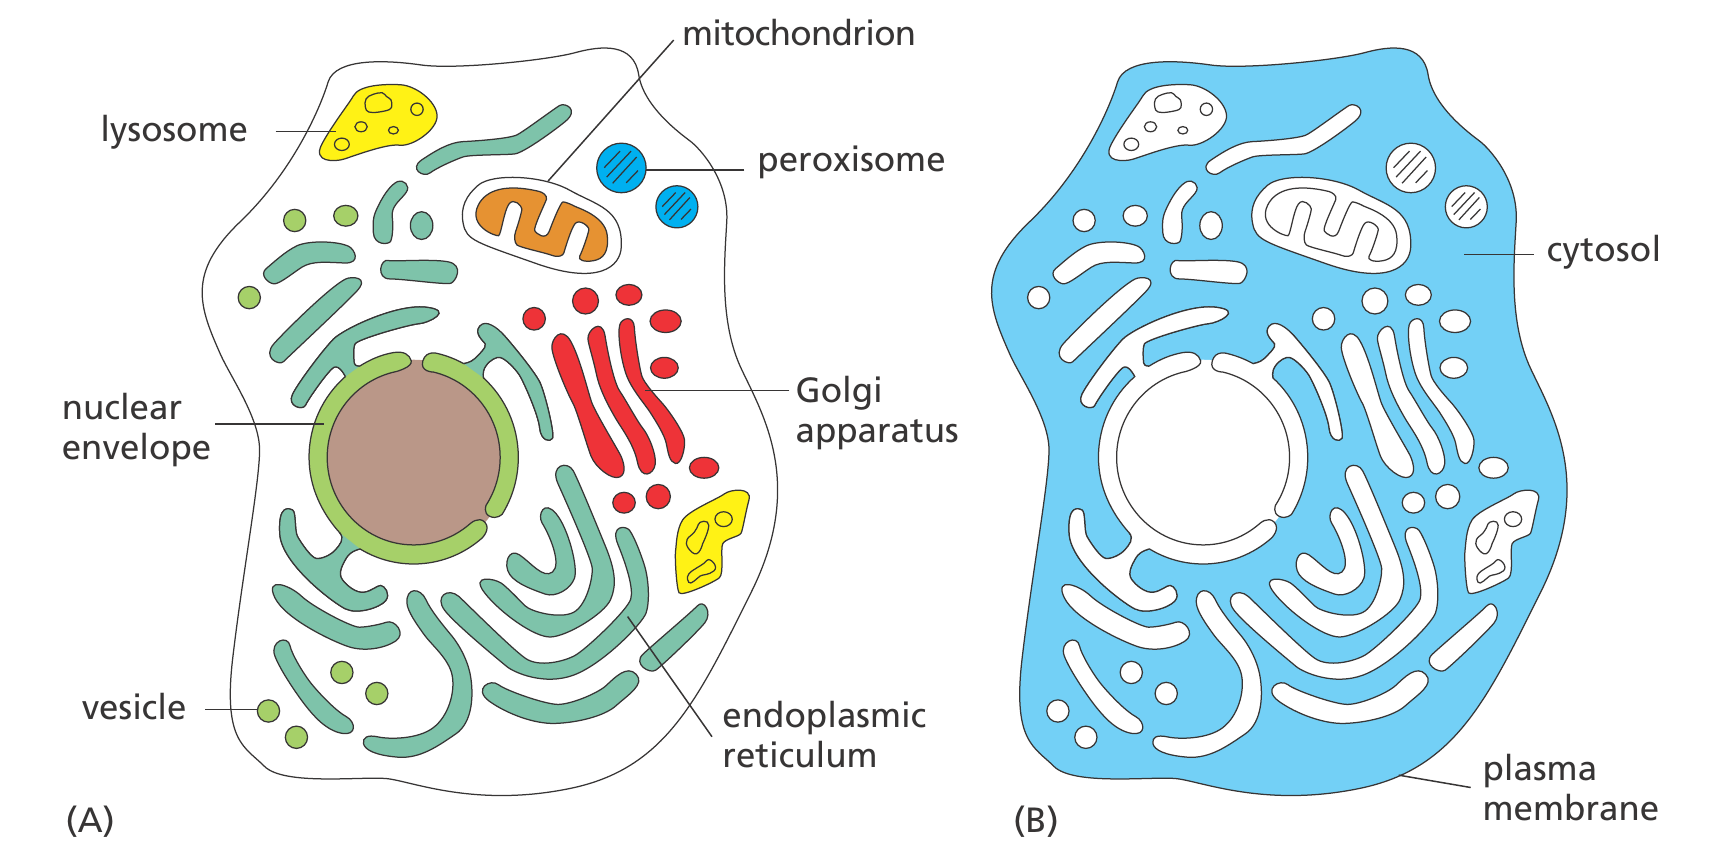
\includegraphics[width=1.0\linewidth]{cellpic_2.png}
		\caption{Composite cell showing various important and common internal cell structures. Most of the volume within the cell is occupied by the cytosol fluid. Figure courtesy of Essential Cell Biology, Alberts, 3rd.}
		\label{fig:cellpic_2.png}
	\end{figure}

	Each cell is enclosed by a plasma membrane that separates the cell contents from the surrounding environment. The inside of the cell is mostly composed of a gel-like substance called cytoplasm that is a dense arrangement of proteins, organelles, and other molecules, suspended in a watery fluid called cytosol. The dense crowding of molecules and organelles results in frequent physical interactions which promotes high metabolic efficiency \citep{ap}. All of the fluid inside the cell may be referred to as intracellular fluid or simply, cellular fluid (CF).
	
	The CF is separated from the extracellular fluid (ECF) by the cell/plasma membrane. This membrane is a phospholipid bilayer with various embedded macromolecular structures. Each phospholipid molecule is amphiphatic, having both a hydrophobic and hydrophilic region. A collection of phospholipid molecules will naturally arrange themselves into a bilayer that does not allow water, polar molecules, or ions to pass through easily. However, water and other molecules or ions need to traverse this membrane and the water transporting task is accomplished by aquaporin gated channel proteins. Aquaporins facilitate the passive diffusion of water through the plasma membrane, between the intracellular and extracellular regions. \citep{ap}.
	
	%These proteins belong to a larger class of proteins called integral membrane bound proteins; some of which act as transporters of various types of molecules or signal transducers.
	
	%Overall, most of the cytosol is water and the viscosity of the cytoplasm is approximately the same as pure water, although the diffusion of small molecules is approximately four times slower than in pure water, due mostly to collisions with the large numbers of macromolecules in the cytosol.

\subsection{Tissues}
	In a multicellular organism, there are several levels of biological organization. A cell is the lowest level of organization that is considered living; tissues are the next higher level of organization and are composed of cells similar in structure and function. This ensemble of cells resides in an extracellular matrix (ECM); a medium containing water, fibrous and adhesive proteins, glycoproteins, and other molecules. The ECM varies in composition between different tissues, but providing structural support and facilitating cell-to-cell communication are common functions of the ECM. In some cells, the cytoplasm is more viscous than the extracellular matrix \citep{cr-biology}. At the cellular level some tissues are relatively organized.
	
	In this project, a simple tissue model was constructed based on some basic defining characteristics of real cells and tissues. The simple tissue model consisted homogeneous spaces, specifically more viscous intracellular regions and less viscous extracellular regions separated by a passive semi-permeable boundary. All of the cells in a model were of the same dimensions and repeated in series.











%Simulation is the imitation of the operation of a real-world process or system over time.[1] The act of simulating something first requires that a model be developed; this model represents the key characteristics or behaviors/functions of the selected physical or abstract system or process. The model represents the system itself, whereas the simulation represents the operation of the system over time.
%
%
%All simulations start with a model. Since the objective of this thesis was to analyze the unbiased diffusion of water molecules in a simple cell or tissue, a model needed to be constructed. It was reasonable to select 
%
%A particular cell or tissue to model is that eukary, any organism that contains . Perhaps the most important defining feature of these eukaryotic cells is that they have membrane-bound organelles and a well defined nucleus. 
%
%First, in order to simulate the diffusion process, a model needed to be constructed. The simple models chosen reflect the basic conditions that might exist in most eukaryotic cells---that is---they contain different compartmental regions separated by semi-permeable membranes.
%
% is intended to imitate of the operation of a real-world process or system over time
%Computers provide an ideal `experimental ground' for simulations that would not be easily feasible or even possible using traditional experimental approaches.
%
%A simple cell model may be used for an approximative analysis of particle diffusion in both 1D and 2D systems.
%
%In the case where the domain of the cell is homogenous (i.e. no internal structures), the calculated effective diffusion coefficient $ D_eff $ is equal to the diffusion coefficient as set in the simulation program parameters. 
%
%As previously mentioned, the goals of this project were to construct a simple-cell model and simulate the process of particle diffusion, under the constraints of absolute boundaries and semi-permeable barriers.
%
%
%
%
%
%
%
%
%
%
%
%
%\section{A sample introduction}
%
%This is just an example, but I wanted to show you some common things to do with Latex.
%
%\subsection{A subsection example}
%
%For of all, here's an equation -- it's the NFW formula, given by \citet{nfw95}, and looks like
%\begin{equation}
%	\label{eq:nfw}
%	\rho(r) = \frac{\rho_s}{r / r_s (1 + r / r_s)^2},
%\end{equation}
%where $\rho_s$ and $r_s$ are a characteristic density and scale radius, respectively.
%
%Now, I can reference that equation later, since it's labelled properly; it's equation (\ref{eq:nfw}).  Notice that I cited a paper above; I could do that in a different way like this \citep{nfw95}.
%
%Just one other quick thing:  figures.  There's one below, and again it's properly labelled.  It's Figure \ref{fig:intro_density}.
%
%\begin{figure}
%\begin{center}
%	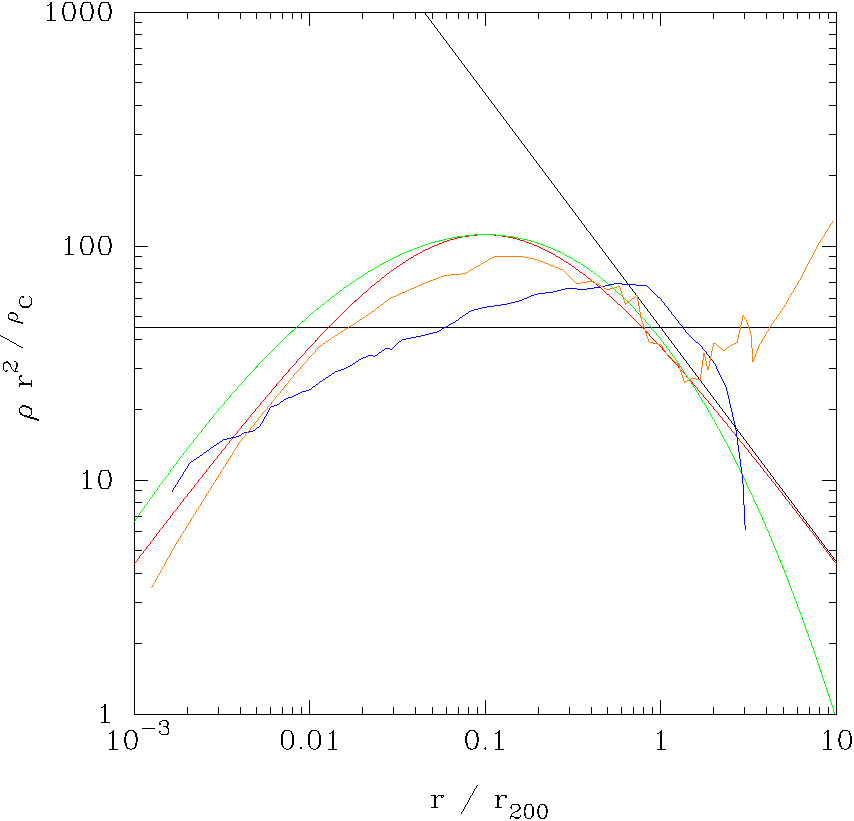
\includegraphics[scale=0.8]{intro_density.pdf}
%\end{center}
%	\caption[Density profiles of various models]{Density profiles, shown as $\rho r^2$ to better highlight the differences, of various models.  }
%	\label{fig:intro_density}
%\end{figure}